\documentclass{article}

\usepackage{fullpage}

\usepackage{graphicx}
\usepackage{wrapfig}

\usepackage[utf8]{inputenc}

\ifdefined\english
\usepackage[english]{babel}
\fi
\ifdefined\spanish
\usepackage[spanish]{babel}
\fi
\ifdefined\french
\usepackage[french]{babel}
\fi

\usepackage{fontspec}
\setmainfont{Open Sans}
\setsansfont{IBM Plex Sans}
\setmonofont{IBM Plex Mono}

\usepackage[hidelinks]{hyperref}

\hypersetup{
    colorlinks,
    urlcolor={blue!80!black}
}

\usepackage{amsmath,amssymb}

\usepackage{fontawesome}
\usepackage[misc]{ifsym}

\setlength{\parindent}{0pt}

\usepackage{sectsty}
\sectionfont{\fontsize{12}{15}\sffamily\bfseries}

\usepackage[dvipsnames]{xcolor}

\newcommand{\biling}[3]{\ifdefined\english#1\fi\ifdefined\spanish#2\fi\ifdefined\french#3\fi}

% % % % % % % % % % % % % % % % % % % % % % % % % % % % % % % % % % % % % % % %

\ifdefined\english
\newcommand{\UES}{University of El~Salvador}
\fi
\ifdefined\spanish
\newcommand{\UES}{Universidad de El~Salvador}
\fi
\ifdefined\french
\newcommand{\UES}{Université de El~Salvador}
\fi

% % % % % % % % % % % % % % % % % % % % % % % % % % % % % % % % % % % % % % % %

\ifdefined\english
\newcommand{\forundergrads}{for undergraduate students}
\fi
\ifdefined\spanish
\newcommand{\forundergrads}{para la licenciatura}
\fi
\ifdefined\french
\newcommand{\forundergrads}{pour licence}
\fi

% % % % % % % % % % % % % % % % % % % % % % % % % % % % % % % % % % % % % % % %

\ifdefined\english
\newcommand{\formsc}{for master students}
\fi
\ifdefined\spanish
\newcommand{\formsc}{para la maestría}
\fi
\ifdefined\french
\newcommand{\formsc}{pour master}
\fi

% % % % % % % % % % % % % % % % % % % % % % % % % % % % % % % % % % % % % % % %

\ifdefined\french
\renewcommand{\baselinestretch}{1.25}
\fi

\begin{document}

{\flushright\noindent\emph{\biling{Updated:}{Actualizado:}{Mise à jour:} \biling{April 2021}{abril de 2021}{avril 2021}}

}

\begin{center}
{\LARGE\sffamily\bf ALEXEY BESHENOV}

\vspace{0.5em}

\faPhoneSquare{} (+52)~473\,139\,4002 \quad
\faGlobe{} \href{https://cadadr.org/}{cadadr.org} \quad
\faEnvelope{} \href{mailto:cadadr@gmail.com}{cadadr@gmail.com} \\

\vspace{0.5em}

Presa del Falcón \# 129, Celaya, 38010, Guanajuato, Gto., \biling{Mexico}{México}{Mexique}

\vspace{1em}

\rule{14cm}{1pt}

\end{center}

\vspace{1em}

% \begin{picture}(1,1) \put(400,-100){\hbox{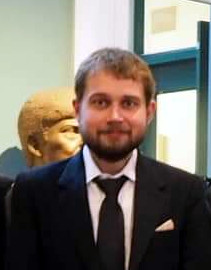
\includegraphics[width=2.5cm]{me.jpg}}} \end{picture}

\noindent \textbf{\biling{Birth date}{Fecha de nacimiento}{Date de naissance}}: \biling{February 24 1989}{24 de febrero de 1989}{24 février 1989}, \biling{USSR}{URSS}{URSS} \\
\textbf{\biling{Citizenship}{Ciudadanía}{Citoyenneté}}: \biling{Russian}{ruso}{russe}

{\color{RoyalBlue}\section*{\biling{ACADEMIC INTERESTS}{INTERESES ACADÉMICOS}{INTÉRÊTS ACADÉMIQUES}}}

\begin{itemize}
\item\biling{algebraic geometry}{geometría algebraica}{géométrie algébrique}
\item \biling{number theory}{teoría de números}{théorie des nombres}
\item \biling{special values of zeta functions}{valores especiales de funciones zeta}{valeurs spéciales des fonctions zêta}
\item \biling{Weil-étale cohomology}{cohomología Weil-étale}{cohomologie Weil-étale}
\item \biling{motivic cohomology}{cohomología motívica}{cohomologie motivique}
\end{itemize}
  
\vspace{1em}

{\color{RoyalBlue}\section*{\biling{EDUCATION}{EDUCACIÓN}{FORMATION}}}

\begin{itemize}
\item \textbf{2014--2018}: \textbf{\biling{University of Bordeaux}{Universidad de Burdeos}{Université de Bordeaux}}\biling{ (France)}{ (Francia)}{},
  \textbf{\biling{Leiden University}{Universidad de Leiden}{Université de Leyde}} (\biling{Netherlands}{Países Bajos}{Pays-Bas}).

  \biling{ALGANT DOC Program}{Programa ALGANT DOC}{Programme ALGANT DOC}, \biling{European Union scholarship}{beca de la Unión Europea}{bourse de l'Union européenne}.

  \textbf{\biling{PhD in mathematics}{Doctor en matemáticas}{Docteur en mathématiques}}.

  \biling{Thesis}{Tesis}{Thèse} \biling{``}{<<}{<<}Zeta-values of arithmetic schemes at negative integers and Weil-étale cohomology\biling{''}{>>}{>>},\\
  \biling{supervised by}{dirigida por}{dirigé par} Baptiste Morin (\biling{Bordeaux}{Burdeos}{Bordeaux}) \biling{and}{y}{et} Bas Edixhoven (\biling{Leiden}{Leiden}{Leyde}).

  \biling{Defense}{Defensa}{Soutenance}: \biling{Leiden}{Leiden}{Leyde}, \biling{December 10, 2018}{10 de diciembre de 2018}{10 décembre 2018}.

  \biling{Referees}{Jurado}{Rapporteurs}:
  S.~Lichtenbaum (\biling{Brown University}{Universidad de Brown}{Université de Brown}),
  N.~Ramachandran (\biling{University of Maryland}{Universidad de Maryland}{Université de Maryland}).

\iffalse
  \biling{Examining committee}{Jurado}:
  P.~Cassou-Noguès (Université de Bordeaux),
  Ph.~Cassou-Noguès (Université de Bordeaux),
  D.~Holmes (Universiteit Leiden)
  R.~de Jeu (Vrije Universiteit Amsterdam),
  W.~van der Kallen (Universiteit Utrecht),
  H.~Lenstra (Universiteit Leiden),
  P.~Stevenhagen (Universiteit Leiden).
\fi

\item \textbf{2012--2014}: \textbf{\biling{University of Milan}{Universidad de Milán}{Université de Milan}} (\biling{Italy}{Italia}{Italie}),
  \textbf{\biling{University of Bordeaux}{Universidad de Burdeos}{Université de Bordeaux}}\biling{ (France)}{(Francia)}{}.

  \biling{ALGANT Master Program}{Programa ALGANT Master}{Programme ALGANT Master}, \biling{European Union scholarship}{beca de la Unión Europea}{bourse de l'Union européenne}.

  \textbf{\biling{MSc in Mathematics}{Maestro en Ciencias con orientación en matemáticas}{Obtention du Master de mathématique}}.

  \biling{MSc thesis}{Tesis de maestría}{Mémoire}
  \biling{on algebraic K theory}{sobre la teoría K algebraica}{sur la K-théorie algébrique},
  \biling{supervised by}{dirigida por}{dirigé par} Boas Erez (\biling{Bordeaux}{Burdeos}{Bordeaux}).

\item \textbf{2010--2012}: \biling{University of the Russian Academy of Sciences}{Universidad de la Academia de Ciencias de Rusia}{Université de l'Académie des sciences de Russie},
  \biling{Saint Petersburg}{San Petersburgo}{Saint-Pétersbourg}, \biling{Department of Mathematics and Computer Science}{Facultad de matemáticas e informática}{Département de mathématiques et d'informatique}.

  \textbf{\biling{MSc in theoretical computer science}{Maestro en Ciencias con orientación en informática teórica}{Obtention du Master d'informatique théorique}},
  diploma cum laude.

  \biling{Thesis advisor}{Director de tesis}{Directeur de mémoire}: Dmitrii Pasechnik.

  \iffalse
\item \textbf{2006--2010}: \biling{Lipetsk State University}{Universidad Estatal de Lipetsk}, \biling{Russia}{Rusia}.

  \textbf{\biling{BSc in computer science and software engineering}{Licenciado en ciencias de computación y programación}},
  diploma cum laude.
  \fi

\end{itemize}

\pagebreak

{\color{RoyalBlue}\section*{\biling{WORK EXPERIENCE}{EXPERIENCIA PROFESIONAL}{EXPÉRIENCE PROFESSIONNELLE}}}

\begin{itemize}
\item \textbf{\biling{October}{Octubre de}{Octobre} 2019 -- \biling{November}{noviembre de}{novembre} 2020}:
  \textbf{\biling{Center for Research in Mathematics}{Centro de Investigación en Matemáticas}{Centre de recherche en mathématiques} (CIMAT)},
  Guanajuato, \biling{Mexico}{México}{Mexique}, \textbf{\biling{visiting researcher}{investigador invitado}{chercheur invité}}.

  \biling{Hosts}{Anfitriones}{Hôtes}: Xavier Gómez Mont, Pedro Luis del Ángel.

\item \textbf{\biling{February}{Febrero de}{Février} 2018 -- \biling{August}{agosto de}{août} 2019}:
  \UES,
  \biling{Natural Sciences Faculty, School of Mathematics}{Facultad de Ciencias Naturales, Escuela de Matemáticas}{Faculté des sciences naturelles, École de mathématiques},
  \textbf{\biling{visiting professor}{profesor invitado}{professeur invité}}.

  \biling{Colaboration with the Ministry of Education of}{Colaboración con el Ministerio de Educación de}{Collaboration avec le ministère de l'Éducation de} El~Salvador,
  \biling{to support the master program in pure mathematics}{con el fin de apoyar el programa de maestría en matemáticas puras}{dans le but de soutenir le programme de master en mathématiques pures}.
  \biling{Lectures for master and bachelor students}{Clases para estudiantes de maestría y licenciatura}{Cours pour étudiants en master et licence},
  \biling{editing of}{redacción de}{édition de}
  \href{https://cadadr.org/san-salvador/}{\biling{teaching materials}{materiales didácticos}{matériel didactique}}, etc.
\end{itemize}

{\color{RoyalBlue}\section*{\biling{TALKS}{CONFERENCIAS}{CONFÉRENCES}}}

\begin{itemize}
\item \textbf{\biling{May}{Mayo de}{Mai} 2021}:
  Seminar on $\mathbb{A}^1$-topology, motives and K-theory,
  \biling{Saint Petersburg}{San Petersburgo}{Saint-Pétersbourg}
  (\biling{online}{en línea}{en ligne})

\item \textbf{\biling{March}{Marzo de}{Mars} 2021}:
  \biling{Number theory seminar}{Seminario de la teoría de números}{Séminaire de théorie des nombres} UAM-ICMAT,
  Madrid (\biling{online}{en línea}{en ligne})

\item \textbf{\biling{February}{Febrero de}{Février} 2020}: Coloquio Oaxaqueño de Matemáticas,
  IMUNAM, Oaxaca

\item \textbf{\biling{December}{Diciembre de}{Décembre} 2019}: First IMSA Conference,
  IMUNAM/CINVESTAV, \biling{Mexico City}{CDMX}{Mexico}

\item \textbf{\biling{November}{Noviembre de}{Novembre} 2019}: Universidad Autónoma de Zacatecas
  (\biling{three talks}{tres conferencias}{trois conférences})

\item \textbf{\biling{October}{Octubre de}{Octobre} 2019}: \biling{XIII Algebra and Topology Workshop}{XIII Taller de Álgebra y Topología}{XIII${}^{\text{e}}$ atelier d'algèbre et topologie},
  IMUNAM, Cuernavaca

\item \textbf{\biling{October}{Octubre de}{Octobre} 2019}: \biling{Algebraic geometry seminar}{Seminario de geometría algebraica}{Séminaire de géométrie algébrique},
  CIMAT, Guanajuato

\item \textbf{\biling{May}{Mayo de}{Mai} 2019}: \biling{Samuel Gitler Conference}{Conferencias Samuel Gitler}{Conférences Samuel Gitler},
  CINVESTAV, \biling{Mexico City}{CDMX}{Mexico}

\item \textbf{\biling{December}{Diciembre de}{Décembre} 2017}:
  \biling{Algebra, geometry and number theory seminar}{Seminario de álgebra, geometría y teoría de números}{Séminaire d'algèbre, géométrie et théorie des nombres}, \biling{Ldeiden}{Leiden}{Leyde}
\end{itemize}

{\color{RoyalBlue}\section*{\biling{MATHEMATICAL WRITING}{TEXTOS MATEMÁTICOS}{TEXTES MATHÉMATIQUES}}}

\begin{itemize}
\item Alexey Beshenov, Margaret Bilu, Yuri Bilu, Purusottam Rath,
  \emph{Rational points on analytic varieties},
  EMS Surv. Math. Sci. 2 (2015), no. 1, 109–130.

  \url{https://doi.org/10.4171/EMSS/10}

\item Alexey Beshenov,
  \emph{Zeta-values of arithmetic schemes at negative integers and Weil-étale cohomology},
  \biling{PhD thesis}{tesis doctoral}{thèse de doctorat}, \biling{Leiden}{Leiden}{Leyde}, \biling{December}{diciembre}{décembre} 2018.

  \url{https://openaccess.leidenuniv.nl/handle/1887/68224}

\item Alexey Beshenov,
  \emph{Weil-étale cohomology for arbitrary arithmetic schemes and $n < 0$.
    Part I: Construction of Weil-étale complexes},
  2020, \biling{preprint}{prepublicación}{prépublication} (arXiv:2012.11034),
  \biling{submitted for publication}{sometido a publicación}{soumis pour publication}.

  \url{https://arxiv.org/abs/2012.11034}

\item Alexey Beshenov,
  \emph{Weil-étale cohomology for arbitrary arithmetic schemes and $n < 0$.
    Part II: The special value conjecture},
  2021, \biling{preprint}{prepublicación}{prépublication} (arXiv:2102.12114).

  \url{https://arxiv.org/abs/2102.12114}

\item Alexey Beshenov,
  \emph{Zeta-values of one-dimensional arithmetic schemes at $n < 0$},
  2021, \biling{in preparation}{en preparación}{en préparation}.

  \url{https://cadadr.org/papers/1-dim-schemes.pdf}
\end{itemize}

\pagebreak

{\color{RoyalBlue}\section*{\biling{TEACHING EXPERIENCE}{EXPERIENCIA DOCENTE}{ENSEIGNEMENT}}}

\noindent\textbf{\biling{One-semester courses}{Cursos semestrales}{Cours d'un semestre}}

\vspace{0.5em}

\begin{itemize}
\item \textbf{\biling{Fall}{Otoño de}{Automne} 2020}:
  \href{https://cadadr.org/cimat-tna/}{\textbf{\biling{Algebraic number theory}{Teoría algebraica de números}{Théorie algébrique des nombres}}},
  \biling{Master program in pure mathematics}{maestría en matemáticas básicas}{master en mathématiques pures},
  CIMAT, Guanajuato.

\item \textbf{\biling{Spring}{Primavera de}{Printemps} 2019}:
  \href{https://cadadr.org/san-salvador/2019-groebner/}{\textbf{\biling{Computational commutative algebra (Gröbner bases)}{Álgebra conmutativa computacional (bases de Gröbner)}{Algèbre commutative computationnelle (bases de Gröbner)}}}
  \formsc, \UES.

\item \textbf{\biling{Spring}{Primavera de}{Printemps} 2019}:
  \href{https://cadadr.org/san-salvador/2019-algebra/}{\textbf{\biling{Algebra}{Álgebra}{Algèbre} I (\biling{rings and groups}{anillos y grupos}{anneaux et groupes})}}
  \forundergrads, \UES.

\item \textbf{\biling{Spring}{Primavera de}{Printemps} 2018}:
  \href{https://cadadr.org/san-salvador/2018-08-algebra-conmutativa/}{\textbf{\biling{Commutative algebra}{Álgebra conmutativa}{Algèbre commutative}}}
  \formsc, \UES.

\item \textbf{\biling{Fall}{Otoño de}{Automne} 2018}:
  \href{https://cadadr.org/san-salvador/2018-algebra/}{\textbf{\biling{Algebra}{Álgebra}{Algèbre} II (\biling{rings and fields}{anillos y campos}{anneaux et corps})}}
  \forundergrads, \UES.

\item \textbf{\biling{Spring}{Primavera de}{Printemps} 2018}:
  \href{https://cadadr.org/san-salvador/2018-algebra/}{\textbf{\biling{Algebra}{Álgebra}{Algèbre} I (\biling{groups}{grupos}{groupes})}}
  \forundergrads, \UES.
\end{itemize}

\noindent\textbf{\biling{Minicourses}{Minicursos}{Mini-cours}}

\begin{itemize}
\item \textbf{\biling{Fall}{Otoño de}{Automne} 2019}:
  \href{https://cadadr.org/cimat-zeta/}{\textbf{\biling{Around arithmetic zeta functions}{En torno de las funciones zeta aritméticas}{Autour des fonctions zêta arithmétiques}}},
  CIMAT, Guanajuato.

\item \textbf{\biling{August}{Agosto de}{Août} 2019}:
  \href{https://cadadr.org/san-salvador/2019-esquemas/}{\textbf{\biling{Scheme theory}{Teoría de esquemas}{Théorie des schémas}}}
  \formsc, \UES.

\item \textbf{\biling{November}{Noviembre de}{Novembre} 2018}:
  \href{https://cadadr.org/san-salvador/2018-cp-tne/reciprocidad-cuadratica.pdf}{\textbf{\biling{Quadratic reciprocity law}{La ley de reciprocidad cuadrática}{Loi de réciprocité quadratique}}}
  \forundergrads, \UES.

\item \textbf{\biling{July}{Julio de}{Juillet} 2018}:
  \href{https://cadadr.org/san-salvador/2018-07-reciprocidad/reciprocidad.pdf}{\textbf{\biling{Reciprocity laws from Gauss to Artin}{Las leyes de reciprocidad de Gauss a Artin}{Lois de réciprocité de Gauss à Artin}}},
  \UES.

\item \textbf{\biling{June}{Junio de}{Juin} 2018}:
  \href{https://cadadr.org/san-salvador/2018-06-categorias/}{\textbf{\biling{Category theory}{Teoría de categorías}{Théorie des catégories}}}
  \formsc, \UES.

\item \textbf{\biling{April}{Abril de}{Avril} 2018}:
  \href{https://cadadr.org/san-salvador/2018-04-numeros-p-adicos/}{\textbf{\biling{p-adic numbers}{Números p-ádicos}{Nombres p-adiques}}}
  \formsc, \UES.

\item \textbf{\biling{February}{Febrero de}{Février} 2018}:
  \href{https://cadadr.org/san-salvador/2017-02-bernoulli/}{\textbf{\biling{Bernoulli numbers}{Números de Bernoulli}{Nombres de Bernoulli}}},
  \UES.

\item \textbf{\biling{August--september}{Agosto–septiembre de}{Août--septembre} 2016}:
  \href{https://cadadr.org/san-salvador/2016-08-homo/}{\textbf{\biling{Homological algebra}{Álgebra homológica}{Algèbre homologique}}},
  \UES.
\end{itemize}

{\color{RoyalBlue}\section*{\biling{LANGUAGES}{IDIOMAS}{LANGUES}}}

\biling{Russian}{Ruso}{Russe} (\biling{native}{nativo}{natif});
\biling{Spanish}{español}{espagnol},
\biling{English}{inglés}{anglais} (\biling{fluent}{fluido}{courant});
\biling{French}{francés}{français},
\biling{Italian}{italiano}{italien} (\biling{intermediate}{intermedio}{intermédiaire}).

\vspace{1em}

{\color{RoyalBlue}\section*{\biling{COMPUTER SKILLS}{CONOCIMIENTOS INFORMÁTICOS}{COMPÉTENCES INFORMATIQUES}}}

GNU/Linux,
LaTeX,
\biling{programming}{programación}{programmation},
\biling{computer algebra systems}{sistemas de álgebra computacional}{systèmes d'algèbre informatique}:
PARI/GP,
Sage,
Macaulay2,
GAP4.

\vspace{1em}

{\color{RoyalBlue}\section*{\biling{REFERENCES}{REFERENCIAS}{RÉFÉRENCES}}}

\begin{itemize}
\item \href{https://www.math.leidenuniv.nl/~edix/}{Bas Edixhoven} (\biling{Leiden University}{Universidad de Leiden}{Université de Leyde})
\item \href{http://www.math.caltech.edu/~flach/}{Matthias Flach} (Caltech)
\item \href{https://www.math.u-bordeaux.fr/~bmorin/}{Baptiste Morin} (\biling{University of Bordeaux}{Universidad de Burdeos}{Université de Bordeaux})
\item \href{https://www.math.umd.edu/~atma/}{Niranjan Ramachandran} (\biling{University of Maryland}{Universidad de Maryland}{Université de Maryland})
\end{itemize}

\end{document}
